% Provenance (never printed): see sources/outline_sources.md (Year 2: oceanic islands; growth,
% flank collapse and erosion of volcanic islands; reefs and atolls; subsidence). Hawaiian
% stages, slides, subsidence and drowned reefs after Clague and Sherrod (2014, USGS PP 1801
% ch. 3) and Denlinger and Morgan (2014, ch. 4); the Nuuanu slide after the ODP Leg 200 report;
% the Enewetak holes after Ladd and Schlanger (1960, USGS PP 260-Y); Kure after the NOAA
% monument pages; the depth--age law from the Book 2 and Book 3 rows. Curves and the invented
% Petrel island from figdata/bachelor-2/islands.py; exercise and problem values in the Book 4
% scratch calculator calc/ch17.py.
\chapter{大洋岛屿}\label{ch:b2:oceanic-islands}

1952 年，在西太平洋埃内韦塔克\omterm{def:b2:oceanic-islands:reefs}{环礁}（当时拼作 Eniwetok）的两座岛上，两口钻孔
穿过珊瑚岩，深度超过 \qty{1.2}{km}。
在帕里岛，钻头在 4,158 英尺（\qty{1267}{m}）深处取出新鲜玄武岩岩屑，随后取出一段橄榄玄武岩岩芯。
其上覆盖着始新世的石灰岩，岩中满是造礁珊瑚，这类珊瑚
通常不会生长在深于约 \qty{46}{m} 之处。曾有珊瑚礁生长在一座火山的山肩上，
靠近海平面，而火山在礁体仍不断向上生长的同时，下沉了超过 1 千米。
本章追踪一座\omterm{def:b2:oceanic-islands:stages}{大洋岛屿}的整个一生：它如何生长，其侧翼如何
坍入海中，为何下沉，以及一圈珊瑚如何能比它存在得更久。
% ledger: ls60:enewetak, ics4:eocene

\begin{recall}
\textbf{来自本科一年级分册}：热点、地幔柱、热点轨迹及其年龄递进，
夏威夷–帝王\omterm{def:b2:oceanic-islands:seamount}{海山}链与夏威夷隆起；洋底的深度–年龄关系；珊瑚礁，
即达尔文所描述的\omterm{def:b2:oceanic-islands:reefs}{岸礁}、\omterm{def:b2:oceanic-islands:reefs}{堡礁}和\omterm{def:b2:oceanic-islands:reefs}{环礁}三种形态，以及“跟上生长，否则淹没”的规则；
全球海平面变化，以及末次盛冰期的海平面，比今天低约 \qty{120}{m}。
\textbf{来自中学分册}：盾状火山；海蚀平台。
\textbf{来自\cref{ch:b2:magmatic-series}}：拉斑系列与\omterm{def:b2:magmatic-series:series}{碱性系列}。
\end{recall}

\section{火山岛的生长}\label{sec:b2:oceanic-islands:growth}

夏威夷群岛是本科一年级分册中横跨
北太平洋的\omterm{def:b2:oceanic-islands:seamount}{海山}链最年轻的一端。主岛上共有已知的 19 座盾状火山：15 座高出海面，
3 座没入水下，另有 1 座新生的火山仍在水下。太平洋板块带着它们向西北漂移，
每一座都在热点之上诞生、生长，随着远离热点而衰亡并沉没。这一历程
足够规则，可以划分为若干阶段。
% ledger: cs14:volcanoes

\begin{definition}[大洋岛屿；生长阶段]\label{def:b2:oceanic-islands:stages}
称从洋底隆起、建于大洋岩石圈之上的火山岛为\emph{大洋岛屿}\index{大洋岛屿}。
热点\omterm{def:b2:oceanic-islands:seamount}{海山}链上的岛屿依次经历四个喷发阶段：
一是\emph{前盾状阶段}，为海底碱性熔岩的小规模喷发；
二是\emph{盾状阶段}\index{盾状阶段}，此时火山位于热点之上，拉斑质熔岩
堆积出火山的主体；三是\emph{后盾状阶段}，喷发次数较少且更偏碱性，
覆盖在盾状火山之上；经过一段停歇后，四是\emph{复活阶段}，喷发稀少、
规模小，属碱性喷发。此后，侵蚀与沉降成为主导。
\end{definition}
% ledger: usgs14:hawaii-stages, cs14:rejuvenated

各阶段随热量供应而变化。最年轻的火山洛伊希位于基拉韦厄峰顶以南 \qty{54}{km}，
其顶部仍在海面以下 \qty{975}{m}，却已高出周围海底 \qty{2.5}{km}；
其最老的熔岩为碱性。\omterm{def:b2:oceanic-islands:stages}{盾状阶段}时，火山位于
热点之上，获得的供应最为充足。据估计，每座夏威夷火山在此阶段喷出的熔岩约占其最终体积的 80 至
\qty{95}{\percent}，多数在最初的 1 至 \qty{2}{Ma} 内完成。
此阶段后期，喷发速率下降为原来的十分之一。浅层\omterm{def:b2:magma-emplacement:magma}{岩浆}储库位于 1
至 \qty{7}{km} 深处，已无法维持活动，但位于 20 至 \qty{30}{km} 处的较小储库仍然保留。
熔岩重新转为碱性，因为较低的熔融程度使之如此，
如\cref{ch:b2:magmatic-series}所示。复活阶段在经过不足 0.5
至 \qty{2.0}{Ma} 的停歇后出现。它可以是一到两次喷发，也可能持续很久：在尼豪，它自 2.2
至 \qty{0.4}{Ma}，在考艾则自 \qty{3.5}{Ma} 起延续至今。
% ledger: cs14:loihi, usgs14:hawaii-stages, cs14:rejuvenated

体积极为庞大。莫纳罗亚的体积估计约为 \qty{74000}{km^3}。当重新划定它与基拉韦厄的边界，使基拉韦厄仅保留约
\qty{10000}{km^3}，则莫纳罗亚的份额升至 \qty{95600}{km^3}。年轻的洛伊希拥有
\qty{1700}{km^3}。自 \qty{81}{Ma} 以来，整条\omterm{def:b2:oceanic-islands:seamount}{海山}链的总量约为
\qty{2e6}{km^3}；若以每年 \qty{0.07}{km^3} 的喷发速率对整段历史积分，结果将接近其三倍。载荷之大，足以使
板块弯曲：岛屿之下的洋壳被压低达 \qty{5}{km}，形成一条称为夏威夷周缘凹陷的槽，
并在数百千米外隆起一个低矮的拱状带，即夏威夷拱。
板块在载荷下如何弯曲，在本科三年级分册中讨论。这里的凹陷之所以重要，
是因为岛屿的大部分碎屑最终汇集于此。
% ledger: cs14:volumes, cs14:loihi, cs14:moat

\begin{omfigure}
\centering
\begin{tikzpicture}[x=0.95cm, y=0.95cm, font=\footnotesize]
% schematic, not to scale (vertical exaggeration about 10). Sea level y = 0; sea floor
% y = -1.6 - 0.0625 (16 - x), deepening with the age of the plate to the left.
\fill[omSea!45] (0,0) -- (16,0) -- (16,-1.6) -- (0,-2.6) -- cycle;
\fill[black!18] (0,-2.6) -- (16,-1.6) -- (16,-3.1) -- (0,-3.1) -- cycle;
\draw[black!60] (0,-2.6) -- (16,-1.6);
\draw[omSea!60!black] (0,0) -- (16,0);
\node[anchor=south, font=\scriptsize] at (8.7,0) {海平面};
% (a) shield stage over the hotspot
\fill[lith basalt, draw=black!70] (12.6,-1.8125) -- (13.9,0.75) -- (14.3,0.9) -- (14.7,0.75) -- (16,-1.6) -- cycle;
% (b) eroded island with a fringing reef (valleys notched in the summit)
\fill[lith basalt, draw=black!70] (9.2,-2.025) -- (10.1,0.15) -- (10.3,0.35) -- (10.45,0.2) -- (10.6,0.45) -- (10.8,0.25) -- (11.0,0.3) -- (11.2,0.1) -- (12.0,-1.85) -- cycle;
\fill[lith reef limestone, draw=black!70] (10.038,0) -- (9.976,-0.15) -- (9.80,0) -- cycle;
\fill[lith reef limestone, draw=black!70] (11.241,0) -- (11.303,-0.15) -- (11.46,0) -- cycle;
% (c) barrier reef around a smaller island, a lagoon between
\fill[lith basalt, draw=black!70] (5.8,-2.2375) -- (7.0,0.2) -- (8.2,-2.0875) -- cycle;
\fill[lith reef limestone, draw=black!70] (6.384,-1.05) -- (6.42,0) -- (6.60,0) -- (6.62,-0.45) -- (6.680,-0.45) -- cycle;
\fill[lith reef limestone, draw=black!70] (7.656,-1.05) -- (7.62,0) -- (7.44,0) -- (7.42,-0.45) -- (7.341,-0.45) -- cycle;
% (d) atoll: volcano bevelled and drowned, reef cap with a lagoon
\fill[lith basalt, draw=black!70] (2.7,-2.43125) -- (3.6,-0.55) -- (4.0,-0.55) -- (4.9,-2.29375) -- cycle;
\fill[lith reef limestone, draw=black!70] (3.4325,-0.9) -- (3.47,0) -- (4.14,0) -- (4.1806,-0.9) -- (4.0,-0.55) -- (3.6,-0.55) -- cycle;
\fill[omSea!45] (3.62,-0.15) rectangle (3.99,0);
% (e) guyot: flat top with a drowned reef cap, beyond the Darwin point
\fill[lith basalt, draw=black!70] (0.2,-2.5875) -- (0.9,-0.95) -- (1.7,-0.95) -- (2.4,-2.475) -- cycle;
\fill[lith reef limestone, draw=black!70] (0.9,-0.95) -- (0.96,-0.75) -- (1.64,-0.75) -- (1.7,-0.95) -- cycle;
% Darwin point
\draw[black!70, dashed] (2.55,0.55) -- (2.55,-2.5);
\node[anchor=south, font=\scriptsize] at (2.55,0.55) {达尔文点};
% hotspot and plate motion
\draw[omThm, line width=1.4pt, -{Stealth[length=2.5mm]}] (14.3,-3.9) -- (14.3,-3.15);
\node[anchor=west, font=\scriptsize, text=omThm] at (14.4,-3.7) {热点};
\draw[black, line width=0.8pt, -{Stealth[length=2.5mm]}] (9.5,-2.85) -- (6.5,-2.85);
\node[anchor=west, font=\scriptsize] at (9.6,-2.85) {板块运动};
\node[anchor=west, font=\scriptsize] at (0.1,-2.9) {大洋岩石圈};
% stage labels
\node[align=center, font=\scriptsize] at (14.3,1.45) {(a) 盾状阶段};
\node[align=center, font=\scriptsize] at (10.6,1.3) {(b) 侵蚀岛屿，\\ 岸礁};
\node[align=center, font=\scriptsize] at (7.0,1.45) {(c) 堡礁};
\node[align=center, font=\scriptsize] at (3.8,1.45) {(d) 环礁};
\node[align=center, font=\scriptsize] at (1.3,1.45) {(e) 平顶海山};
\draw[black!60, -{Stealth[length=2mm]}] (13.6,-3.7) -- (0,-3.7);
\node[anchor=south, font=\scriptsize, fill=white, inner sep=1pt] at (7,-3.7) {较老的火山，较老且较深的板块};
\end{tikzpicture}
\par\smallskip{\small 沿热点\omterm{def:b2:oceanic-islands:seamount}{海山}链看\omterm{def:b2:oceanic-islands:stages}{大洋岛屿}的一生（示意图，不按比例，
竖直比例大幅放大）。板块把每座火山带离热点，
（图中向右），火山随之下沉，同时侵蚀不断将其削低。(a)~盾状火山在热点之上
生长。(b)~火山已停止喷发、遭受侵蚀，四周镶有\omterm{def:b2:oceanic-islands:reefs}{岸礁}。(c)~进一步下沉后，
被\omterm{def:b2:oceanic-islands:reefs}{堡礁}环绕，礁后有泻湖。(d)~山顶已没入海面以下，礁盖与
中央有泻湖的\omterm{def:b2:oceanic-islands:reefs}{环礁}在其顶部生长。(e)~被带入水温过低、礁体难以跟上的水域后，
\omterm{def:b2:oceanic-islands:reefs}{环礁}被淹没，以\omterm{def:b2:oceanic-islands:seamount}{平顶海山}的形式沉没。}
\end{omfigure}
% ledger: cs14:volcanoes, cs14:erase, cs14:darwin-point, pmnm:geology

\section{山体侧翼垮塌}\label{sec:b2:oceanic-islands:collapse}

一座高达数千米的火山，由松散的熔岩流和碎屑堆积而成，立于一直延伸入海沟的斜坡之上，
这样的火山并不稳定。1975 年，震级为 7.7 的卡拉帕纳地震
使基拉韦厄火山的南侧斜坡一次性向海方向移动达 \qty{10}{m}，并引发海啸。
1868 年，另一次斜坡移动伴随震级为 7.9 的地震与一场海啸，
造成 46 人死亡。这些斜坡下方的地震剖面显示出一个深部反射界面，人们将其解释为
沿古老洋壳顶部的一个\omterm{def:b2:alpine-orogen:decollement}{滑脱面}，整个斜坡沿此面滑动。通常，
斜坡只是缓慢蠕滑，有时则会失稳崩塌。
% ledger: dm14:flank

\begin{definition}[山体侧翼垮塌；碎屑崩落；滑塌]\label{def:b2:oceanic-islands:collapse}
\emph{山体侧翼垮塌}\index{山体侧翼垮塌}是指火山侧翼的大片区域
发生失稳，在自身重力作用下滑离。当滑动的
块体破碎并快速流散，形成可远远越过火山山麓的块体与碎屑流时，则称为
\emph{碎屑崩落}\index{碎屑崩落}。若其缓慢移动，形成大块体
沿植根于深部\omterm{def:b2:alpine-orogen:decollement}{滑脱面}的断层转动、停留在火山附近的情形，则称为\emph{滑塌}。
\end{definition}

证据埋藏于海面之下。20 世纪 80 年代末，
利用侧扫声呐对夏威夷群岛周围海域的测绘表明，在距岛屿数百千米的深海海底上散布着大量碎屑，
并有由大块分节岩块组成的滑塌体。共有 17 处大型滑坡被识别出，
位于主要岛屿周围，形成于过去 \qty{5}{Ma} 之内。目前已知沿夏威夷海岭、
位于夏威夷岛与中途岛之间的滑坡共 70 处，形成时间跨度为 \qty{30}{Ma}。换言之，
主要岛屿周围至少每 \qty{300}{ka} 便发生一次滑坡。这些统计数字只是下限，因为一座
较年轻的火山可能掩埋较老火山的滑坡疤痕与碎屑，例如尼豪岛的顶部\omterm{def:b2:eruptive-styles:caldera}{破火山口}与裂谷带
已经缺失，且至今未找到相应的沉积物。巨型滑坡似乎最可能发生在火山
生长最快的时期，即从前\omterm{def:b2:oceanic-islands:stages}{盾状阶段}后期到后\omterm{def:b2:oceanic-islands:stages}{盾状阶段}早期，
但此后很长时间仍会继续发生。
% ledger: cs14:slides, dm14:flank

最大的一次是努阿努滑坡，它扯离了瓦胡岛科劳火山的东北侧翼，
形成一场\omterm{def:b2:oceanic-islands:collapse}{碎屑崩落}，覆盖面积达 \qty{23000}{km^2}，向外延伸
离岛超过 \qty{200}{km}。其块体中包括图斯卡卢萨\omterm{def:b2:oceanic-islands:seamount}{海山}，长约 \qty{30}{km}，
宽 \qty{17}{km}，高至少 \qty{2}{km}。崩落体越过深邃的海沟，
沿夏威夷隆起带的斜坡向上攀升了超过 \qty{100}{km}。其年龄估计为 2.1 至
\qty{1.8}{Ma}，接近科劳火山生命的末期或之后；其地表熔岩的年龄为 1.8 至
\qty{2.6}{Ma}。它由几次崩塌形成，以及远离岛屿处的厚度有多大，
仍是未解的问题。
% ledger: odp200:nuuanu

\begin{omfigure}
\centering
\begin{tikzpicture}[x=0.95cm, y=0.95cm, font=\footnotesize]
% schematic section from the summit of an island (left) across the moat to the arch (right);
% not to scale. Sea level y = 0; top of the old oceanic crust, bent down under the island.
\fill[omSea!45] (0,0) -- (15,0) -- (15,-2.2) -- (13.5,-2.12) -- (11,-2.05) -- (8.5,-2.35) -- (6.5,-2.75) -- (5.6,-2.82) -- (4.0,-1.4) -- (2.5,0) -- cycle;
\fill[black!18] (0,-3.05) -- (5.6,-2.82) -- (6.5,-2.75) -- (8.5,-2.35) -- (11,-2.05) -- (13.5,-2.12) -- (15,-2.2) -- (15,-3.6) -- (0,-3.6) -- cycle;
\draw[black!70] (0,-3.05) -- (5.6,-2.82) -- (6.5,-2.75) -- (8.5,-2.35) -- (11,-2.05) -- (13.5,-2.12) -- (15,-2.2);
\draw[omSea!60!black] (0,0) -- (15,0);
\node[anchor=south east, font=\scriptsize] at (15,0) {海平面};
% the volcano: present flank (after collapse) and the lost flank (dashed)
\fill[lith basalt, draw=black!70] (0,1.15) -- (0.8,1.05) -- (1.25,0.95) -- (1.45,0.45) -- (1.75,0.1) -- (2.6,-0.75) -- (3.6,-1.6) -- (4.6,-2.4) -- (5.6,-2.82) -- (0,-3.05) -- cycle;
\draw[black!70, dashed] (1.25,0.95) -- (2.5,0) -- (4.0,-1.4) -- (5.6,-2.82);
\node[font=\scriptsize, align=center, fill=white, inner sep=1pt] at (0.8,-1.6) {火山};
\node[font=\scriptsize, anchor=south west, align=left] at (2.0,0.25) {崩失侧翼 \\ 的疤痕};
% slump: blocks rotated on listric faults rooted in the decollement
\draw[black, line width=0.7pt] (1.45,0.45) .. controls (1.7,-1.4) and (2.4,-2.6) .. (3.6,-2.95);
\draw[black, line width=0.7pt] (2.6,-0.75) .. controls (2.8,-1.8) and (3.3,-2.6) .. (4.4,-2.9);
\draw[omThm, line width=1.1pt] (0.6,-3.03) -- (5.6,-2.82);
\node[anchor=north, font=\scriptsize, text=omThm] at (2.9,-3.05) {滑脱面};
% debris avalanche: hummocky sheet across the moat and up the arch, with blocks
\fill[lith conglomerate, draw=black!70] (4.6,-2.4) -- (5.6,-2.62) -- (6.5,-2.6) -- (8.5,-2.22) -- (11,-1.95) -- (12.6,-2.03) -- (11,-2.05) -- (8.5,-2.35) -- (6.5,-2.75) -- (5.6,-2.82) -- cycle;
\fill[lith basalt, draw=black!70] (7.0,-2.62) -- (7.25,-2.25) -- (7.95,-2.22) -- (8.1,-2.43) -- cycle;
\fill[lith basalt, draw=black!70] (9.3,-2.2) -- (9.45,-2.02) -- (9.75,-2.0) -- (9.85,-2.17) -- cycle;
\fill[lith basalt, draw=black!70] (10.6,-2.05) -- (10.7,-1.93) -- (10.9,-1.92) -- (10.95,-2.03) -- cycle;
\draw[black!70] (7.6,-2.2) -- (7.4,-1.3) node[anchor=south, font=\scriptsize, align=center] {宽数千米的 \\ 块体};
\node[anchor=south, font=\scriptsize, align=center] at (10.3,-1.3) {碎屑崩落};
\draw[black!70] (10.3,-1.3) -- (10.0,-1.98);
\node[font=\scriptsize] at (6.6,-3.2) {海沟};
\node[font=\scriptsize] at (11.6,-2.6) {隆起带};
\node[anchor=west, font=\scriptsize] at (12.6,-3.3) {洋壳};
\draw[black!70] (2.55,-1.55) -- (3.35,-0.6) node[anchor=west, font=\scriptsize, inner sep=1pt] {滑塌};
\draw[black!60, {Stealth[length=2mm]}-{Stealth[length=2mm]}] (5.6,-3.95) -- (12.6,-3.95);
\node[anchor=north, font=\scriptsize] at (9.1,-3.95) {至约 \qty{200}{km}};
\end{tikzpicture}
\par\smallskip{\small \omterm{def:b2:oceanic-islands:stages}{大洋岛屿}的\omterm{def:b2:oceanic-islands:collapse}{山体侧翼垮塌}（示意图，不按比例）。靠近
火山处，滑塌以沿断层转动的块体形式缓慢移动，这些断层植根于\omterm{def:b2:alpine-orogen:decollement}{滑脱面}，该面位于
老洋壳的顶部。\omterm{def:b2:oceanic-islands:collapse}{碎屑崩落}使侧翼脱离、留下疤痕，并以
碎屑席的形式铺展，席上携带数千米宽的块体。努阿努崩落越过海沟，
爬上隆起带，离瓦胡岛超过 \qty{200}{km}。}
\end{omfigure}
% ledger: dm14:flank, odp200:nuuanu, cs14:moat

滑坡落入海中时会把海水推开。在拉奈岛和莫洛凯岛上，杂乱的角砾岩
由珊瑚和熔岩组成，高出海平面可达 \qty{155}{m}，曾被解释为崩塌掀起的巨浪所形成的沉积。
这一解释存在争议。有些作者以岛屿隆升来解释这些沉积，
但拉奈岛以南被淹没的礁体并无此类隆升的迹象。
大约三分之一的夏威夷巨型滑坡属于能掀起巨浪的\omterm{def:b2:oceanic-islands:collapse}{碎屑崩落}。
这类灾害虽罕见却规模极大，如何权衡，留待\cref{ch:b2:geological-hazards}中讨论。
% ledger: cs14:megatsunami

\section{大洋岛屿为何下沉}\label{sec:b2:oceanic-islands:subsidence}

\omterm{def:b2:oceanic-islands:stages}{大洋岛屿}下沉由两个相互重叠的过程造成。第一个是加载：火山
不断生长，其重量将板块压下。这一快速阶段约持续一百万年，
使海岸线与礁体的淹没深度超过一千米。在夏威夷岛西北海岸外，
经测年的被淹没礁体给出的下沉速率为每千年 \qty{2.6}{m}。一座小型
火山在此阶段可能被整体淹没：位于夏威夷岛旁的马胡科纳曾短暂成为岛屿，
现今其山顶位于水下约 \qty{1100}{m}。第二个过程是板块的
冷却，它持续约一亿年，本节将其以
数值形式加以表述。
% ledger: cs14:subsidence, cs14:mahukona

本科一年级分册给出了洋底深度随其年龄 $t$（以 \unit{Ma} 计）增加的规律。
本章采用的形式如下：
\[
d(t) = \qty{2500}{m} + C\sqrt{t}, \qquad C = \qty{350}{m.Ma^{-1/2}}, \qquad 0 \le t \le 70,
\]
对于年龄大于约 \qty{20}{Ma} 的板块，
\[
d(t) = \qty{6400}{m} - \qty{3200}{m}\; e^{-t/62.8}.
\]
两式在 20 至 \qty{50}{Ma} 之间相差约 \qty{20}{m} 以内，并在
\qty{26}{Ma} 处相交。
% ledger: ps77:depth-age (Book 2), parsons:plate-model (Book 3)
% values (islands.py): t_switch 26.27, d_switch 4293.8; root - exp: 20 Myr -7.6, 50 Myr +18.3

\begin{proposition}[岛屿的热沉降]\label{prop:b2:oceanic-islands:sinking}
一座建于年龄为 $t_1$ 的板块上的岛屿，随板块一同移动，并对板块施加一个
不再变化的重量，且不改变其下方板块的冷却，则下沉量为
\[
S = d(t_2) - d(t_1)
\]
截至板块年龄达到 $t_2$ 时，下沉速率为 $\dot S = d'(t)$。对于平方根律，
\[
S = C\left(\sqrt{t_2} - \sqrt{t_1}\right), \qquad \dot S = \frac{C}{2\sqrt t},
\]
对于指数律，$\dot S = (\qty{3200}{m}/\qty{62.8}{Ma})\,e^{-t/62.8}$。在某一给定的
时间区间内，年轻板块所承载的岛屿比老板块下沉得更多。
\end{proposition}

\begin{proof}
比较板块上两根年龄相同的柱体，一根位于岛屿之下，另一根位于
远处的开阔大洋之下。两者以相同方式冷却，因为岛屿不改变板块的冷却，故二者收缩量相同，顶部下降的
量相同。岛屿自身的重量已经平衡且不再变化，故不再增加
任何影响。开阔大洋的柱体下降 $d(t_2) - d(t_1)$，岛屿亦然。对其求导即得
速率。对于最后一个结论：在固定区间 $\Delta$ 内，$C(\sqrt{t_1 + \Delta} -
\sqrt{t_1})$ 随 $t_1$ 增大而减小，因为其导数 $\frac C2\bigl(1/\sqrt{t_1 + \Delta}
- 1/\sqrt{t_1}\bigr)$ 为负。
\end{proof}

本命题有意略去了两点。热点隆起在板块经过时将其抬起，
离开后又使其下沉，这会加剧最年轻岛屿的下沉
（本科一年级分册测量过这一隆起）。另外，火山生长时负荷也在变化，这便是
上文所述的快速阶段。两者结束之后，岛屿便随海底一同下沉。

下沉速率很小。对于 \qty{4}{Ma} 的板块，平方根律给出每百万年 \qty{87.5}{m}，
即每年不到十分之一毫米。对于 \qty{100}{Ma} 的板块，指数律
给出每百万年 \qty{10.4}{m}，即每千年 \qty{0.01}{m}。这正是
沿夏威夷海岭和天皇\omterm{def:b2:oceanic-islands:seamount}{海山}链大部分区段所测得的速率。负荷阶段的速率为
每千年 \qty{2.6}{m}，约快 250 倍。
% ledger: cs14:subsidence; values (islands.py): rate_100 10.37, age_rate10 102.3

\begin{omfigure}
\centering
% figdata/bachelor-2/islands.py part sink
\begin{tikzpicture}
\begin{axis}[width=0.8\linewidth, height=6.2cm, y dir=reverse, xmin=0, xmax=100, ymin=0,
  ymax=3000, xlabel={岛屿建成以来的时间（\unit{Ma}）},
  ylabel={热沉降（\unit{m}）}, tick label style={font=\scriptsize},
  label style={font=\small}, xtick pos=bottom, ytick pos=left]
\addplot[omThm, line width=1pt] table[x=dt_Myr, y=t2] {figdata/out/bachelor-2-islands-sink.dat};
\addplot[orange!80!black, line width=1pt] table[x=dt_Myr, y=t10] {figdata/out/bachelor-2-islands-sink.dat};
\addplot[blue!70!black, line width=1pt] table[x=dt_Myr, y=t30] {figdata/out/bachelor-2-islands-sink.dat};
\addplot[black!45, line width=1pt] table[x=dt_Myr, y=t60] {figdata/out/bachelor-2-islands-sink.dat};
\node[font=\scriptsize, anchor=south east, inner sep=1pt] at (axis cs:99,2470) {板块 \qty{2}{Ma}};
\node[font=\scriptsize, anchor=south east, inner sep=1pt] at (axis cs:99,2140) {\qty{10}{Ma}};
\node[font=\scriptsize, anchor=south east, inner sep=1pt] at (axis cs:99,1380) {\qty{30}{Ma}};
\node[font=\scriptsize, anchor=south east, inner sep=1pt] at (axis cs:99,710) {\qty{60}{Ma}};
\draw[black!50, dashed] (axis cs:0,1267) -- (axis cs:58,1267);
\node[font=\scriptsize, anchor=north west, inner sep=1pt] at (axis cs:1,1300) {恩尼威托克，\qty{1267}{m}};
\end{axis}
\end{tikzpicture}
\par\smallskip{\small 由深度–年龄关系计算得到的、随板块移动的岛屿热沉降，
对应建于板块年龄分别为 2、10、30 和 \qty{60}{Ma} 的岛屿（板块年龄不超过
\qty{26}{Ma} 时采用平方根律，此后采用指数律，两者在此相交）。板块越年轻，岛屿下沉越快
、下沉量越大。虚线标出恩尼威托克下方玄武岩的深度，即
下沉过程中需要为之腾出空间的礁岩厚度。}
\end{omfigure}
% ledger: ps77:depth-age (Book 2), parsons:plate-model (Book 3), ls60:enewetak

\section{礁、环礁与平顶海山}\label{sec:b2:oceanic-islands:reefs}

本科一年级分册用达尔文的解释描述了三种礁的形态，从岛屿边缘的\omterm{def:b2:oceanic-islands:reefs}{岸礁}
到环绕泻湖的珊瑚环，并以一个问题作结：岛屿为何下沉，
下沉多少？上一节已经回答了这个问题。现在可以依据其下方岛屿的
状态来界定这些形态。

\begin{definition}[岸礁；堡礁；环礁]\label{def:b2:oceanic-islands:reefs}
\emph{岸礁}\index{岸礁}是附着于岛屿海岸的礁体，礁与岸之间没有
泻湖，或仅有狭窄而浅的水道相隔。\emph{堡礁}\index{堡礁}
是与海岸被泻湖隔开的礁体，位于一座已经下沉、而礁体仍在向上生长的岛屿的
侧翼。\emph{环礁}\index{环礁}是一圈礁体，圈内有由礁石碎屑构成的低矮小岛，
环绕着一个泻湖，且无火山岩露出海平面：其火山完全位于礁体之下。
\end{definition}

\begin{definition}[海山；平顶海山]\label{def:b2:oceanic-islands:seamount}
\emph{海山}\index{海山}是位于海底的火山，其顶部位于海平面以下，
原因或是它从未露出水面，或是它已经下沉。
\emph{平顶海山}\index{平顶海山}是顶部平坦的海山，其顶部被海浪削平或被礁体覆盖，
此时位于海平面，之后沉没。
\end{definition}

若礁体的顶部保持在海平面，而火山随之下沉，则礁岩堆积的
速度与岛屿下沉的速度相同。于是礁盖的厚度便记录了下沉量。

\begin{proposition}[礁盖的厚度]\label{prop:b2:oceanic-islands:cap}
设岛屿最后的火山岩在板块年龄为 $t_1$ 时降至海平面以下，并设一
礁体自此起始终保持其顶部位于海平面，直至板块年龄达到 $t_2$。若在两时刻之间海平面
相对于地心上升了 $\Delta\eta$，则火山之上的礁盖
厚度为
\[
H = d(t_2) - d(t_1) + \Delta\eta = C\left(\sqrt{t_2} - \sqrt{t_1}\right) + \Delta\eta
\]
厚。其中第二种形式采用平方根律。该厚度不依赖于礁体能够
生长的速率，只要该速率不小于海平面的相对上升速率。
\end{proposition}

\begin{proof}
在 $t_1$ 时刻，火山顶部位于海平面；在 $t_2$ 时刻，它低了 $S = d(t_2) - d(t_1)$
（由\cref{prop:b2:oceanic-islands:sinking}可知），同时海面上升了 $\Delta\eta$。礁体的
顶部在两个时刻都位于海面，其底部即为火山顶部。因此厚度即二者之间的距离
$S + \Delta\eta$。能跟上的礁体始终停留在海面，
因此生长更快的礁体并不会形成更厚的礁盖；跟不上的礁体则落后并被淹没，
这正是本科一年级分册所回顾的规律。
\end{proof}

恩尼威托克\omterm{def:b2:oceanic-islands:reefs}{环礁}证实了这一点。按根号定律，厚度为 \qty{1267}{m} 的礁盖需要 $\sqrt{t_2} - \sqrt{t_1} =
1267/350 = 3.62$：例如，一座火山在板块年龄为 \qty{10}{Ma} 时被削至海平面，
随后被带走，直到板块年龄为 \qty{46}{Ma}。这一时长为 \qty{36}{Ma}，
大致相当于将石灰岩底界的始新世与今天隔开的时间尺度。钻孔还揭示了该命题
未涵盖的内容。淋滤带，即珊瑚文石被溶解或
重结晶之处，记录了\omterm{def:b2:oceanic-islands:reefs}{环礁}顶部高出海面、有雨水落在其上的时期。
海平面随冰期而升降，礁盖在下沉途中多次出露、又被淹没，
且此过程已反复多次。
% ledger: ls60:enewetak, ics4:eocene; calc/ch17.py: (3.162 + 3.620)^2 = 46.0

\begin{history}[钻探环礁，1896--1952]
达尔文的理论作出了一项只能靠钻探来检验的预言：\omterm{def:b2:oceanic-islands:reefs}{环礁}之下应有一厚层浅水礁岩，
覆于火山岩之上。太平洋\omterm{def:b2:oceanic-islands:reefs}{环礁}上的第一个深钻孔
于 1896 至 1898 年在富纳富提钻成，钻至 1,114 英尺，
即 \qty{340}{m}，尚未钻到火山。位于日本以南、冲绳以东的北大东岛上的钻孔
于 1936 年钻至 1,416 英尺；比基尼\omterm{def:b2:oceanic-islands:reefs}{环礁}上的钻孔于 1947 年钻至 2,556 英尺，二者均未钻到火山。恩尼威托克\omterm{def:b2:oceanic-islands:reefs}{环礁}上的钻孔，于
1951 和 1952 年完成，是首次钻到\omterm{def:b2:oceanic-islands:reefs}{环礁}基底的钻孔。在伊卢格拉布，坚硬的基底
于 4,610 英尺处被钻遇；帕里岛上的玄武岩位于 4,158 英尺处，高出 450 英尺，
两者相距 \num{22}~英里。钻探者发现了一座玄武质火山，它高出洋底两英里，
自始新世起便被礁灰岩覆盖。伊卢格拉布在一次热核装置试验中被摧毁，
这发生在钻探结束后不久。
\end{history}
% ledger: ls60:holes, ls60:enewetak

\begin{omfigure}
\centering
% figdata/bachelor-2/islands.py part holes
\begin{tikzpicture}
\begin{axis}[width=0.8\linewidth, height=6.0cm, ybar, bar width=16pt, y dir=reverse, ymin=0,
  ymax=1500, enlarge x limits=0.1, symbolic x coords={Funafuti,Kita-daito-jima,Bikini,Eniwetok-K-1B,Eniwetok-F-1,Eniwetok-E-1},
  xtick=data, xticklabels={{富纳富提 \\1898},{北大东岛 \\1936},{比基尼 \\1947},{恩尼威托克 \\K-1B, 1951},{恩尼威托克 \\F-1, 1952},{恩尼威托克 \\E-1, 1952}},
  xticklabel style={align=center, font=\scriptsize}, ylabel={深度 (\unit{m})},
  tick label style={font=\scriptsize}, label style={font=\small}, xtick pos=bottom, ytick pos=left]
\addplot[fill=omLithLime, draw=black!70] table[x=name, y=td_m] {figdata/out/bachelor-2-islands-holes.dat};
\addplot[only marks, mark=-, mark size=9pt, line width=2.2pt, black, unbounded coords=discard, xshift=0pt]
  table[x=name, y=basalt_m] {figdata/out/bachelor-2-islands-holes.dat};
\end{axis}
\end{tikzpicture}
\par\smallskip{\small 太平洋\omterm{def:b2:oceanic-islands:reefs}{环礁}上钻成的深钻孔，并标出各孔的完成年份：
总深度以柱形表示，恩尼威托克\omterm{def:b2:oceanic-islands:reefs}{环礁}上玄武\omterm{def:b2:magma-emplacement:bodies}{岩基}底的深度以黑色短横线表示
（伊卢格拉布 F-1 之下为 \qty{1405}{m}；帕里岛 E-1 之下为 \qty{1267}{m}）。深度由
钻探报告中的英尺换算而来。}
\end{omfigure}
% ledger: ls60:holes, ls60:enewetak; values (islands.py): td and basalt in m

\begin{inthefield}[钻探环礁]
在恩尼威托克，地质学家将深钻孔布置在靠近泻湖岸边的位置，他们预计那里
的洞穴比礁缘外侧附近少。钻孔大部分为竖直钻进，岩石被磨成
岩屑，由钻井液带出地面。岩屑出现得较晚，因此队员估算了这一滞后，
以便知道每个样品来自哪一深度。在选定的深度，取芯筒取出一段
实心的岩柱。钻探结束后，这些钻孔被用作测量仪器。其中一个钻孔下了套管，
且至 \qty{600}{m} 深处仍为实心岩层，其水位仍随海洋潮汐同步、等幅地涨落，
这说明礁盖的石灰岩多孔，通体充满洞穴。另有人
测量了钻孔中温度恢复平衡的过程。
\end{inthefield}
% ledger: ls60:methods, ls60:casing (F-1 cased to 1,973 ft = 601 m)

礁体不一定会因其所在的岛屿下沉而淹没。珊瑚与珊瑚藻
每年可增长数毫米：在一项现代研究中，以分枝状珊瑚为主的礁体曾以每年 \qty{4.2}{mm}
的速度增长。冷却的
板块每年最多带走十分之一毫米。仅靠热沉降，永远
赶不上健康的礁体。礁体淹没，是因为有其他因素发生变化：板块将其带入
不利于快速生长的较冷水域；海平面上升速度快于礁体所能跟上的速度；或二者同时发生。
% ledger: perry:chagos (Book 3), cs14:darwin-point

\begin{omfigure}
\centering
% figdata/bachelor-2/islands.py part rates; horizontal lines from the ledger rows
\begin{tikzpicture}
\begin{semilogyaxis}[width=0.8\linewidth, height=6.4cm, xmin=0, xmax=150, ymin=0.005, ymax=100,
  xlabel={板块年龄 (\unit{Ma})}, ylabel={速率 (\unit{mm.\text{年}^{-1}})},
  tick label style={font=\scriptsize}, label style={font=\small}, xtick pos=bottom, ytick pos=left]
\addplot[omThm, line width=1.1pt] table[x=t_Myr, y=thermal_mm_yr] {figdata/out/bachelor-2-islands-rates.dat};
\draw[omThm, densely dotted, line width=0.9pt] (axis cs:75,0.01) -- (axis cs:150,0.01);
\node[font=\scriptsize, anchor=south west, inner sep=1pt, text=omThm] at (axis cs:22,0.042) {板块的热沉降};
\node[font=\scriptsize, anchor=south west, inner sep=1pt, text=omThm] at (axis cs:96,0.0108) {实测，夏威夷海岭};
\draw[black!70, line width=0.9pt] (axis cs:0,2.6) -- (axis cs:150,2.6);
\node[font=\scriptsize, anchor=north west, inner sep=1pt] at (axis cs:2,2.6) {载荷，夏威夷岛外侧};
\draw[green!50!black, line width=0.9pt] (axis cs:0,4.2) -- (axis cs:150,4.2);
\node[font=\scriptsize, anchor=south west, inner sep=1pt, text=green!40!black] at (axis cs:2,4.2) {高产礁体的生长};
\draw[blue!70!black, line width=0.9pt] (axis cs:0,12) -- (axis cs:150,12);
\node[font=\scriptsize, anchor=south west, inner sep=1pt, text=blue!70!black] at (axis cs:2,12) {末次冰消期的平均海平面上升};
\draw[blue!70!black, line width=0.9pt, dashed] (axis cs:0,40) -- (axis cs:150,40);
\node[font=\scriptsize, anchor=south west, inner sep=1pt, text=blue!70!black] at (axis cs:2,40) {融冰水脉冲 1A，至少};
\end{semilogyaxis}
\end{tikzpicture}
\par\smallskip{\small 决定礁体能否跟上的速率，采用对数坐标。
板块的热沉降（由深度–年龄关系得出）比礁体生长慢数十至数百倍；
虚线为沿夏威夷海岭大部分区段实测的速率。正在生长的火山在
自身载荷下的沉降，尤其是冰期结束时的海平面上升，与礁体的生长
速率相当，或超过它。}
\end{omfigure}
% ledger: cs14:subsidence, perry:chagos (Book 3), lambeck14:lgm (Book 2), ipcc:lgm-sea (Book 2)

\begin{definition}[达尔文点]\label{def:b2:oceanic-islands:darwin-point}
热点链上的\emph{达尔文点}\index{达尔文点}，是指这样的位置，以及火山诞生之后的
时间：此时礁体的向上生长（在较冷水域中会变慢）
已不足以抵消岛屿的下沉。被带至其外侧的\omterm{def:b2:oceanic-islands:reefs}{环礁}将被淹没，
并成为\omterm{def:b2:oceanic-islands:seamount}{平顶海山}。
\end{definition}

在夏威夷岛链上，礁体在其火山诞生约 \qty{33}{Ma} 后被淹没。库雷\omterm{def:b2:oceanic-islands:reefs}{环礁}位于岛链西北端，
是世界上纬度最高的珊瑚\omterm{def:b2:oceanic-islands:reefs}{环礁}，
正处于\omterm{def:b2:oceanic-islands:darwin-point}{达尔文点}上，其礁体仍略快于\omterm{def:b2:oceanic-islands:reefs}{环礁}的下沉而增长。中途岛与库雷以外的每座
火山均已没入水下，其中大多数为\omterm{def:b2:oceanic-islands:seamount}{平顶海山}。在南部天皇\omterm{def:b2:oceanic-islands:seamount}{海山}链上的高子\omterm{def:b2:oceanic-islands:seamount}{海山}，
碳酸盐沉积自约 50 至 \qty{16}{Ma} 形成。此后，最后的深水珊瑚藻
沉降至其生长下限以下，位于海面以下约 \qty{150}{m} 处。仅有较冷的
水或仅有下沉，都不足以淹没礁体。淹没需要下沉、向北漂入较冷水域、
以及气候的快速变化三者同时作用。
% ledger: cs14:darwin-point, pmnm:kure, pmnm:geology

\begin{omfigure}
\centering
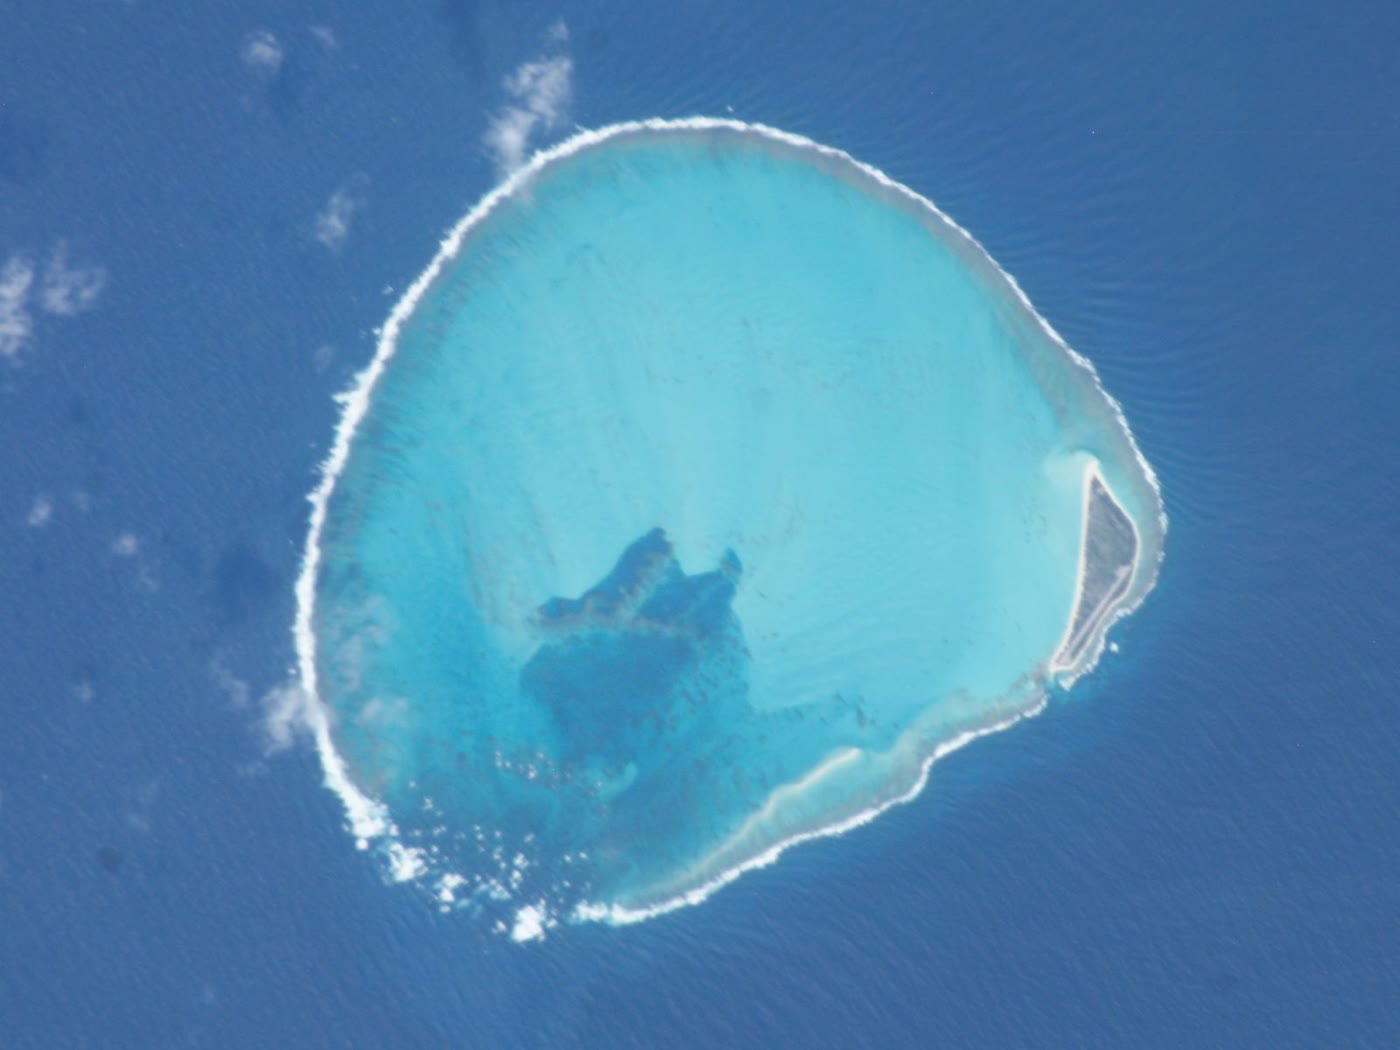
\includegraphics[width=0.52\linewidth]{images/book4/b2-17-kure-atoll.jpg}
\par\smallskip{\small 库雷\omterm{def:b2:oceanic-islands:reefs}{环礁}是最北的珊瑚\omterm{def:b2:oceanic-islands:reefs}{环礁}，由
国际空间站上的宇航员于 2004 年 2 月 22 日拍摄。礁环直径至多约十千米，
环绕一个泻湖；唯一的常年性岛屿格林岛位于礁缘（右侧）。NASA，
公有领域，经维基共享资源。}
\end{omfigure}
% ledger: pmnm:kure (6 miles = 9.7 km)

\section{侵蚀、海平面与岛屿的消亡}\label{sec:b2:oceanic-islands:erosion}

岛屿在下沉的同时也被侵蚀。高大的岛屿会拦截信风：在夏威夷火山的迎风坡，
某些地方一年降雨超过 \qty{9}{m}。河流在不到一百万年内便切出深深的峡谷，
如夏威夷岛上的科哈拉。
一些曾被认为仅由侵蚀形成的巨大悬崖，如莫洛凯岛北部的海崖，
如今被解释为巨型滑坡的后壁，此后又经后退。海浪冲击海岸，
并在其周围海平面处削出海蚀平台。侵蚀与下沉共同作用，
在约 \qty{15}{Ma} 内使海面以上的火山岩荡然无存。年龄与之相近的加德纳尖峰，
是岛链中火山岩仍露出水面的最古老岛屿。其西北方向之外，
只剩沙岛、\omterm{def:b2:oceanic-islands:reefs}{环礁}和沉没的火山。
% ledger: cs14:erosion, cs14:erase

在此过程中，海平面并非静止不动。末次盛冰期时，海平面约比今天低
\qty{120}{m}。那时岛屿的海岸位于其斜坡较低处，而如今环绕岛屿的礁体
当时尚为陆地。冰川融化时，海平面平均每千年上升 \qty{12}{m}，
在主要去冰期内（自 16.5 至 \qty{8.2}{ka}）。融水脉冲 1A 期间，
海平面每年至少上升 \qty{40}{mm}。沉降中的火山上的礁体必须跟上这两次上升。
夏威夷岛西北海岸外，至少六座被淹没的礁体在斜坡上构成
阶梯，最老者最深。每座礁体都在海岸处生长，遇海面上升便落后，
并被年轻岛屿的负荷带着下沉。火山一旦下沉超过
约 \qty{125}{m}（即冰期海平面的变幅），便不会重新浮出水面。
% ledger: usgs:lgm (Book 1), lambeck14:lgm (Book 2), cs14:erase, cs14:subsidence

拱曲也可能反向作用。瓦胡岛坐落于较年轻岛屿负荷所形成的隆起之上，
并已略有抬升：末次间冰期的礁体年龄为 133 至 \qty{115}{ka}，
环绕全岛出露；一座年龄约为 \qty{334}{ka} 的礁体如今高出海平面 \qty{21}{m}。
因此，\omterm{def:b2:oceanic-islands:stages}{大洋岛屿}的消亡过程记录于其岩石与礁体之中。熔岩将其堆高，
滑坡与降雨将其削低，海浪将其削平，板块将其带向深处，而礁体在
地表保持其位置，直至冷水与上升的海平面连它一并淹没。
% ledger: cs14:arch

\section*{练习}\label{sec:b2:oceanic-islands:exercises}

除另有说明外，练习数据如下：深度–年龄关系 $d = \qty{2500}{m} + C\sqrt t$，其中
$C = \qty{350}{m.Ma^{-1/2}}$，适用于 $0 \le t \le \qty{70}{Ma}$；超过 \qty{20}{Ma} 时，$d = \qty{6400}{m} -
\qty{3200}{m}\,e^{-t/62.8}$；$1~\text{英尺} = \qty{0.3048}{m}$，$1~\text{英寻}
= \qty{1.8288}{m}$，$1~\text{英里} = \qty{1.609}{km}$；礁体生长速率至多为 \qty{4.2}{mm.\text{年}^{-1}}。

\begin{exercise}[$\star$]\label{exo:b2:oceanic-islands:1}
指出每座火山所处的阶段：(a) 一座\omterm{def:b2:oceanic-islands:seamount}{海山}，峰顶位于海面以下 \qty{975}{m}，喷发碱性熔岩；
(b) 位于热点之上的火山，高速喷发拉斑质熔岩；(c) 一座已灭绝的火山，其最后的熔岩流
比岛屿主体更富碱性，覆盖于盾状火山体之上；(d) 一座岛屿，经过 \qty{2}{Ma} 的平静期后，
又有若干小型碱性火山口通道开启；(e) 环绕泻湖的礁环，
视野内不见火山岩。
\end{exercise}

\begin{exercise}[$\star$]\label{exo:b2:oceanic-islands:2}
火山建于年龄为 \qty{9}{Ma} 的板块上。(a) 其周围海底深度为多少？(b) 当板块
年龄达到 \qty{25}{Ma} 时，火山将下沉多少？(c) 此时下沉速率为多少？
\end{exercise}

\begin{exercise}[$\star$]\label{exo:b2:oceanic-islands:3}
过去 \qty{5}{Ma} 内，夏威夷主要岛屿周围形成了十七次大型滑坡，
沿夏威夷海岭，在 \qty{30}{Ma} 内形成七十次。(a) 求两种情形下
两次滑坡之间的平均间隔；(b) 为什么这两个结果都只是真实间隔的上限？
\end{exercise}

\begin{exercise}[$\star$]\label{exo:b2:oceanic-islands:4}
在埃尼威托克，一个钻孔在 4,158 英尺深处遇到玄武岩，另一个钻孔在 4,610 英尺深处
遇到坚硬基底；石灰岩底部的礁珊瑚生存深度不超过 150 英尺。(a) 将
这三个深度换算为米。(b) 帕里岛下火山的顶部自第一批礁体
生长以来至少下沉了多少？(c) 石灰岩底部属始新世，年龄至少为
\qty{33.9}{Ma}。平均下沉速率的最大可能值是多少？
\end{exercise}

\begin{exercise}[$\star\star$]\label{exo:b2:oceanic-islands:5}
(a) 分别以 \unit{m} 每 \unit{Ma} 和 \unit{mm.\text{年}^{-1}} 为单位，求
年龄为 4、25 和 \qty{49}{Ma} 的板块上岛屿的热沉降速率。(b) 高产礁体的生长速率
能比其中最快者快多少倍？(c) 夏威夷岛外的负荷阶段，
其速率为 \qty{2.6}{m} 每千年，这比最快者快多少倍？
\end{exercise}

\begin{exercise}[$\star\star$]\label{exo:b2:oceanic-islands:6}
(a) 用指数律求年龄为 \qty{100}{Ma} 的板块的下沉速率，单位为 \unit{m}
每千年，并与沿
夏威夷海岭测得的 \qty{0.01}{m} 每千年相比较。(b) 板块年龄为多少时，速率恰为 \qty{10}{m.Ma^{-1}}？(c) 验证
两种定律对年龄为 \qty{25}{Ma} 的板块给出的深度几乎相同。
\end{exercise}

\begin{exercise}[$\star\star$]\label{exo:b2:oceanic-islands:7}
夏威夷的礁体在其火山诞生约 \qty{33}{Ma} 后被淹没，火山活动
沿岛链以 \qty{8.6}{cm.\text{年}^{-1}} 的速度迁移。(a) 礁体淹没时，岛屿距热点多远？
(b) 中途岛是年龄为 \qty{27.7}{Ma} 的\omterm{def:b2:oceanic-islands:reefs}{环礁}，它仍有活礁，是否合理？
(c) 库雷位于中途岛之外 55 英里处。估计其年龄，并判断它是否
接近\omterm{def:b2:oceanic-islands:darwin-point}{达尔文点}。
\end{exercise}

\begin{exercise}[$\star\star$]\label{exo:b2:oceanic-islands:8}
在努阿努\omterm{def:b2:oceanic-islands:collapse}{碎屑崩落}中，塔斯卡卢萨\omterm{def:b2:oceanic-islands:seamount}{海山}是一块长约 \qty{30}{km}、
宽 \qty{17}{km}、高至少 \qty{2}{km} 的岩块。(a) 以这些尺寸为边的长方体，其体积为多少？
若以同底、同高的棱锥计，其体积又为多少？(b) 与基拉韦厄火山的
体积 \qty{10000}{km^3} 相比较。(c) 崩落体覆盖面积为 \qty{23000}{km^2}。若其平均
厚为 \qty{100}{m}（此为假设，远离瓦胡岛处的厚度鲜有了解），则其
体积应为多少？
\end{exercise}

\begin{exercise}[$\star\star$]\label{exo:b2:oceanic-islands:9}
夏威夷岛外的斜坡在火山负荷作用下，每千年下沉 \qty{2.6}{m}。
(a) 使海岸线内移 \qty{1}{km} 需要多长时间？(b) 以 \qty{4.2}{mm.\text{年}^{-1}} 速率生长的礁体
位于该斜坡上。海平面稳定时，它能否跟上？(c) 在主要去冰期（自 16.5 至 \qty{8.2}{ka}）内，
海平面平均以 \qty{12}{mm.\text{年}^{-1}} 的速率上升。若礁体始于海面，则期末
礁顶深度为多少？(d) 对位于一座不再下沉的古老火山上的礁体，
同样求出其结果。
\end{exercise}

\begin{exercise}[$\star\star\star$]\label{exo:b2:oceanic-islands:10}
(a) 证明：在固定区间 $\Delta$ 内，根定律使岛屿的下沉量随其所在板块年龄增大而减小。
(b) 计算在 \qty{20}{Ma} 内，生于洋脊处的岛屿与生于年龄为 \qty{50}{Ma} 板块上的岛屿各自的下沉量。
(c) 洋脊下的板块温度很高，根定律在
$t = 0$ 处给出无穷大的速率。这对有限区间内的下沉量是否构成问题？请说明理由。
\end{exercise}

\begin{exercise}[$\star\star\star$]\label{exo:b2:oceanic-islands:11}
一座\omterm{def:b2:oceanic-islands:reefs}{环礁}以 \qty{30}{m.Ma^{-1}} 的速率下沉，海平面随冰期旋回大约波动 \qty{120}{m}，
旋回周期约为 \qty{100}{ka}。(a) \omterm{def:b2:oceanic-islands:reefs}{环礁}在一个旋回内下沉多少？(b) 在冰期低海面时，
\omterm{def:b2:oceanic-islands:reefs}{环礁}顶部高出海面多少？此时礁岩会发生什么变化？
(c) \omterm{def:b2:oceanic-islands:reefs}{环礁}下沉完整的 \qty{120}{m} 需要多少个旋回？
(d) 解释在 Enewetak 钻孔中发现的淋滤带，以及为什么
\cref{prop:b2:oceanic-islands:cap} 在长时间尺度上仍给出礁盖的厚度。
\end{exercise}

\begin{exercise}[$\star\star\star$]\label{exo:b2:oceanic-islands:12}
一座\omterm{def:b2:oceanic-islands:reefs}{环礁}在板块年龄为 \qty{50}{Ma} 时被淹没：礁体落后，
顶部止于最深珊瑚藻的生长极限，即海面下 \qty{150}{m}。(a) 按指数定律，
在板块年龄达到 \qty{120}{Ma} 之前还将下沉多少？(b) 此时
\omterm{def:b2:oceanic-islands:seamount}{平顶海山}顶部的深度为多少？(c) 靠近 Enewetak 的一座\omterm{def:b2:oceanic-islands:seamount}{平顶海山}，其顶部位于 700 英寻处。换算并加以比较。
(d) 说出两个理由，解释实际\omterm{def:b2:oceanic-islands:seamount}{平顶海山}的深度为何可能比此估计更深或更浅。
\end{exercise}

\begin{problem}[{周末问题——从火山到环礁}]\label{pb:b2:oceanic-islands:1}
虚构的佩特雷尔岛形成于板块年龄为 \qty{10}{Ma} 的热点之上。其火山是
一座基底半径为 \qty{50}{km} 的锥体。生长结束时，其顶峰高出海平面 \qty{1000}{m}。
其最后的火山岩在 \qty{12}{Ma} 后没入海平面以下。此后，礁体的顶部保持在海平面，
直至板块年龄达到 \qty{70}{Ma}，此时\omterm{def:b2:oceanic-islands:reefs}{环礁}越过
\omterm{def:b2:oceanic-islands:darwin-point}{达尔文点}。请使用习题中给出的深度–年龄关系（\qty{70}{Ma} 以内用根定律，
超出部分用指数定律），礁体生长速率取 \qty{4.2}{mm.\text{年}^{-1}}，并利用本章数据。
除第 8 至 10 题外，海平面均取为常数。深度取整至米。

\noindent\textbf{第一部分——生长。}
\begin{enumerate}
  \item 佩特雷尔岛诞生处的海底深度为多少？
  \item 生长结束时，忽略荷载作用下海底的
        下沉，火山高出该海底的高度为多少？
  \item 求该锥体的体积。
  \item 若其中 \qty{85}{\percent} 在 \qty{1}{Ma} 的\omterm{def:b2:oceanic-islands:stages}{盾状阶段}内喷出，平均喷发速率为
        多少？并与今日基拉韦厄火山的供给量作比较，后者约为
        每年 \qty{0.1}{km^3}。
  \item 若莫纳罗亚火山体积为 \qty{95600}{km^3}，需要多少座佩特雷尔火山才能抵得上它？
  \item 锥体主体由拉斑质还是碱性熔岩构成？又是哪一类覆盖其上？
\end{enumerate}

\noindent\textbf{第二部分——加载与淹没的礁体。}
\begin{enumerate}[resume]
  \item 生长期间，荷载使年轻岛屿在 \qty{1}{Ma} 内下沉 \qty{1}{km}，其平均速率为
        多少？它与在夏威夷岛外测得的
        每千年 \qty{2.6}{m} 相比如何？
  \item 此阶段礁体在海岸上生长，海平面保持稳定。礁体能否跟上，
        余量有多大？
  \item 随后海平面以 \qty{12}{mm.\text{年}^{-1}} 上升，礁体每年
        落后多少？
  \item 礁顶达到最深生长极限 \qty{150}{m} 需要多久？
        这在岛屿斜坡上留下了什么？
\end{enumerate}

\noindent\textbf{第三部分——下沉与侵蚀。}
\begin{enumerate}[resume]
  \item 当其最后的火山岩没入海面时（此时板块年龄为
        \qty{22}{Ma}），佩特雷尔岛已下沉多少？
  \item 在顶部 \qty{1000}{m} 的高度中，侵蚀移除了多少？平均速率为多少？
  \item 生长结束时与顶部消失时，佩特雷尔岛的下沉速率各为多少？
  \item 此时其周围海底的深度为多少？
  \item 将其所用的 \qty{12}{Ma} 与夏威夷群岛的 \qty{15}{Ma} 作比较，并
        说明高耸的夏威夷岛为何存在得更久。
  \item 说出除降雨和河流之外，还有哪两种过程能将岛屿从海面以上移除。
  \item 顶部消失前不久，环绕佩特雷尔岛的是哪种礁？
\end{enumerate}

\noindent\textbf{第四部分——\omterm{def:b2:oceanic-islands:reefs}{环礁}与\omterm{def:b2:oceanic-islands:seamount}{平顶海山}。}
\begin{enumerate}[resume]
  \item 板块年龄为 \qty{70}{Ma} 时，礁盖厚度为多少？
  \item 这需要怎样的平均礁体生长速率？它比礁体
        可达到的生长速率小多少倍？
  \item 将礁盖厚度与 Enewetak 之下玄武岩的深度作比较。
  \item \omterm{def:b2:oceanic-islands:reefs}{环礁}越过\omterm{def:b2:oceanic-islands:darwin-point}{达尔文点}时，其周围海底的深度为多少？
  \item 按指数定律，被淹没的\omterm{def:b2:oceanic-islands:reefs}{环礁}在板块年龄达到
        \qty{120}{Ma} 之前还将下沉多少？
  \item 若礁顶在淹没时停于 \qty{150}{m}，则此时\omterm{def:b2:oceanic-islands:seamount}{平顶海山}的
        顶部深度为多少？
  \item 综上，佩特雷尔\omterm{def:b2:oceanic-islands:reefs}{环礁}的礁盖厚度为多少？
\end{enumerate}
\end{problem}
